\section{Introduction}

This paper will examine a mathematics theory I’ve been working on for quite some time. I call it the study of ``N-Units Away Curves.'' I actually first discovered this fascinating little enigma in my doodles when I was perhaps only five or six years old. The particular little geometric phenomenon I discovered was really interesting, and I couldn’t explain it at the time. All these years later as a grown man and mathematician, it gives me a nice feeling of catharsis to finally rigorously address this question and comprehend its mysteries.

\begin{figure}[h!]
  \centering
  \label{intro-1} 
  \begin{minipage}[b]{0.3\linewidth}
    \centering
    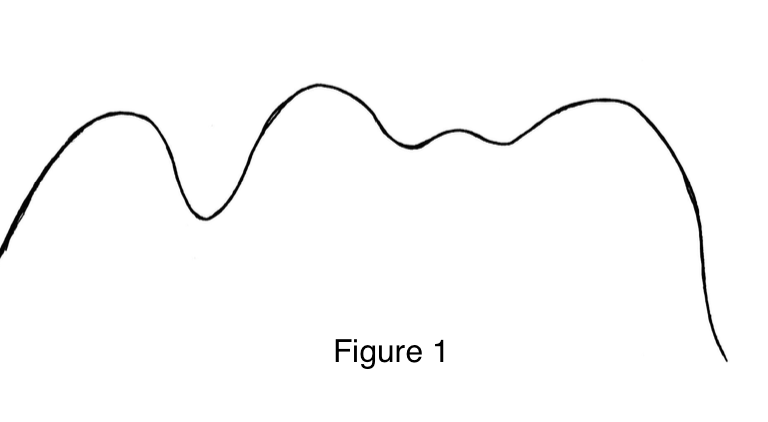
\includegraphics[width=.9\linewidth]{intro_img/Fig 1.png} 
    \caption{A squiggle} 
    \label{fig:fig1}
    \vspace{4ex}
  \end{minipage} % end 
  \begin{minipage}[b]{0.3\linewidth}
    \centering
    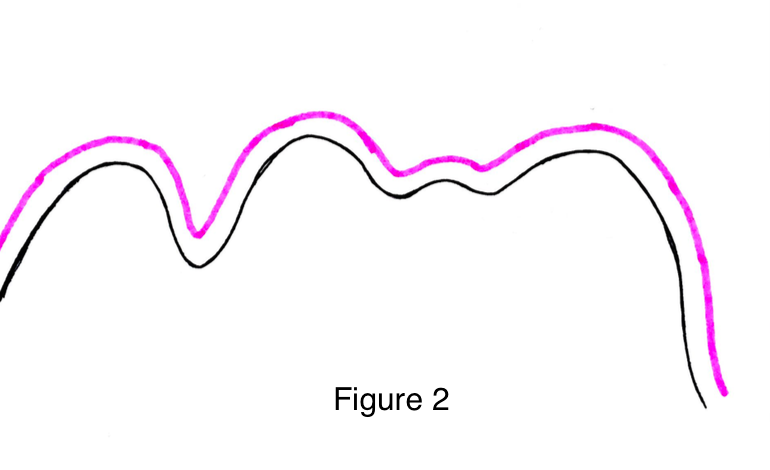
\includegraphics[width=.9\linewidth]{intro_img/Fig 2.png} 
    \caption{Caption} 
    \label{fig:fig2}
    \vspace{4ex}
  \end{minipage} % end
  \begin{minipage}[b]{0.3\linewidth}
    \centering
    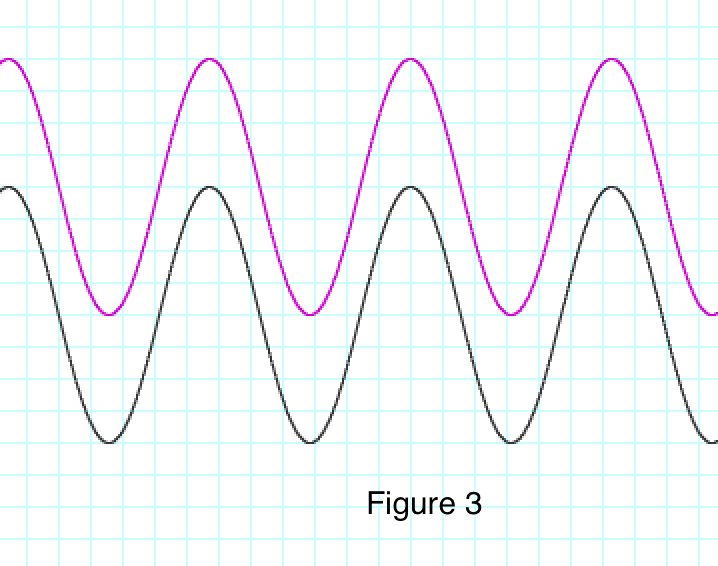
\includegraphics[width=.9\linewidth]{intro_img/Fig 3.png} 
    \caption{Caption} 
    \label{fig:fig3}
    \vspace{4ex}
  \end{minipage} % end
  \begin{minipage}[b]{0.3\linewidth}
    \centering
    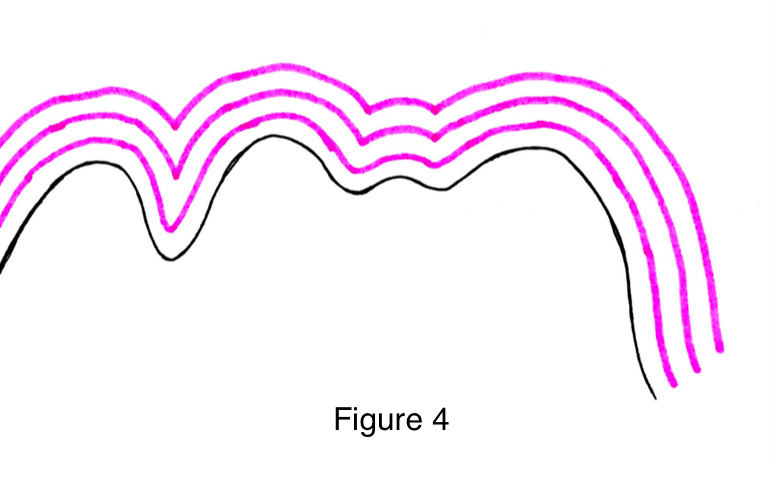
\includegraphics[width=.9\linewidth]{intro_img/Fig 4.png} 
    \caption{Caption} 
    \label{fig:fig4}
    \vspace{4ex}
  \end{minipage} % end
\end{figure}

As a little kid I discovered the following phenomenon in my doodles... Draw a curve. Any curve. A squiggle on a page will suffice. An example is provided in Figure \ref{fig:fig1}. It felt natural as a little kid to then draw another curve next to it that was the same distance away from the first at all points. (Fig \ref{fig:fig2}) Note that this is very different than what is more typically encountered in mathematics: two curves like $y = sin(4x)$ and $y = sin(4x) + 1$ are such that the second curve always remains 1 unit away from the first specifically in the $y$-direction (Fig \ref{fig:fig3})... This is not what my little kid self meant at all. Imagine rolling a marble through the little “tube” that lies between $y = sin(4x)$ and $y = sin(4x) + 1$. At some points the little tube is wide and fat, at other points the tube gets very skinny and narrow. This is fundamentally different from the idea my kid self wanted us to do which was to take a curve and draw a $2^{nd}$ one next to it that would create a perfect nice little tube... a tube with the same diameter at all spots (see Figure \ref{fig:fig2}).



As a child doodling, it seemed natural to then repeat the process and draw another curve that lay the same distance away from this new curve. I’d repeat the process a whole bunch of times (Fig \ref{fig:fig4}), but then something curious always happened. I had started with a smooth curve. But as I ran the process again and again, inevitably the curves always “got pointy.” At first I assumed this was due to inaccuracies in my drawings, so I set out (crayons in hand) to draw these curves very accurately and was absolutely flabbergasted to discover that the phenomenon remained! What in the world was the reason for that? Why were the curves “getting pointy”? A mystery was born. Many years passed by, and eventually I found myself enrolled in a high school Calculus class. One day we learned about inverse trigonometric functions (specifically ) and a little while later it dawned on me... I finally had the mathematical tools I needed to further study these “curves that lie N units away”! My intent was now to figure out how to program my Pacific Tech Graphing Calculator to be able to take in an arbitrary function $y = f(x)$ and graph the associated curve that lies exactly N units away at all points. I wanted to be able to finally see exactly what these curves looked like. I did so in the following manner.